\section{Propagator Interface}\label{sec:system}

We now turn to the implementation of theory propagation in \clingo~5
and detail the structure of its interface depicted in Figure~\ref{fig:interface}.
%
\begin{figure}
  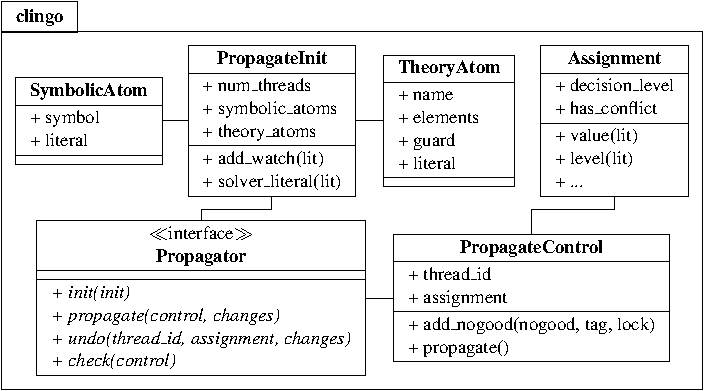
\includegraphics[width=\textwidth]{figures/python-interface}
  \caption{Class diagram of \clingo's (theory) propagator interface\label{fig:interface}}
\end{figure}
%
% To begin with,
The interface \code{Propagator} has to be implemented by each custom propagator.
After registering such a propagator with \clingo,
its functions are called during initialization and search as indicated % in the algorithm
in Figure~\ref{fig:cdcl}.
%
Function \code{Propagator.init}%
\footnote{For brevity, we below drop the qualification \code{Propagator} and use its function names unqualified.}
is called once before solving (Line~(\ref{fig:cdcl:init}) in Figure~\ref{fig:cdcl})
to allow for initializing data structures used during theory propagation.
It is invoked with a \code{PropagateInit} object providing access to symbolic (\code{SymbolicAtom}) as well as theory (\code{TheoryAtom}) atoms.
Both kinds of atoms are associated with program literals,\footnote{Program literals are also used in the \aspif\ format (see~\ref{sec:aspif}).} % ~\cite{gekakaosscwa16b}
which are in turn associated with solver literals.%
\footnote{Note that \clasp's preprocessor might associate a positive or even negative solver literal with multiple atoms.}
Program as well as solver literals are identified by non-zero integers, where positive and negative numbers represent positive or  negative literals, respectively.
In order to get notified about assignment changes, a propagator can set up watches on solver literals during initialization.

During search, function \codeClass{Propagator}{propagate} is called with a \code{PropagateControl} object
and a (non-empty) list of watched literals that got assigned in the recent round of unit propagation (Line~(\ref{fig:cdcl:propagate}) in Figure~\ref{fig:cdcl}).
The \code{PropagateControl} object can be used to inspect the current assignment, record nogoods, and trigger unit propagation.
Furthermore, to support multi-threaded solving,
its \code{thread\_id} property identifies the currently active thread,
each of which can be viewed as an independent instance of the CDCL algorithm in Figure~\ref{fig:cdcl}.%
%Hence, thread-specific state has to be associated with the \code{thread\_id}.
\footnote{%
Depending on the configuration of \clasp, threads can communicate with each other.
For example, some of the recorded nogoods can be shared.
This is transparent from the perspective of theory propagators.}
%
Function \codeClass{Propagator}{undo} is the counterpart of \codeClass{Propagator}{propagate}
and called whenever the solver retracts assignments to watched literals (Line~(\ref{fig:cdcl:undo}) in Figure~\ref{fig:cdcl}).
In addition to the list of watched literals that have been retracted (in chronological order),
it receives the identifier and the assignment of the active thread.
%
Finally, function \codeClass{Propagator}{check} is similar to \codeClass{Propagator}{propagate},
yet invoked without a list of changes.
Instead, it is (only) called on total assignments
(Line~(\ref{fig:cdcl:check}) in Figure~\ref{fig:cdcl}), independently of watches.
%
Overriding the empty default implementations of propagator methods is optional.
% Implementing the propagator methods, which default to empty implementations, is optional. % that does nothing.
For brevity, we below focus on implementations of the methods in \python,
while \lua\ or \C\ could be used as well.

For illustration,
consider Listing~\ref{prg:pigeon:propagator} giving a propagator for (half of) the pigeon-hole problem.
%
\lstinputlisting[linerange={1-10,12-39},float=t,mathescape=true,escapeinside={\#(}{\#)},basicstyle={\ttfamily\small},label={prg:pigeon:propagator},caption={Propagator for the pigeon-hole problem},language=clingo]{example/pigeon-py.lp}
%
Although this setting is constructed, it showcases central aspects
that are also relevant when implementing more complex propagators,
e.g., the \code{Pigeonator} is both stateful and can be used with multiple threads.
%
The underlying ASP encoding is given in Line~\ref{prg:pigeon:prop:rule1}:
A (choice) rule generates solution candidates by placing each of the $p$ pigeons in exactly one among $h$ holes.
While the rule commented out in Line~\ref{prg:pigeon:prop:rule2} would ensure that there is at most one pigeon per hole,
this constraint is handled by the \code{Pigeonator} class
implementing the \code{Propagator} interface (except for \code{check}) in Lines~\ref{prg:pigeon:prop:begin-init}--\ref{prg:pigeon:prop:end-undo}.
Whenever two pigeons are placed in the same hole, it adds a binary nogood forbidding the placement.
To this end,
it maintains data structures for, given a newly placed pigeon,
detecting whether there is a conflict.
%
More precisely, the propagator has two data members:
The \code{self.place} dictionary in Line~\ref{prg:pigeon:prop:member-place} maps solver literals
for \code{place}$/2$ atoms to their corresponding holes,
and the \code{self.state} list in Line~\ref{prg:pigeon:prop:member-state} stores for each solver thread its current placement of pigeons
as a mapping from holes to true solver literals for \code{place}$/2$ atoms.

Function \codeClass{Pigeonator}{init} in Lines~\ref{prg:pigeon:prop:begin-init}--\ref{prg:pigeon:prop:end-init}
sets up watches as well as the dictionaries in \code{self.place} and \code{self.state}.
%
To this end,
it traverses (symbolic) atoms over \code{place}$/2$ in Lines~\ref{prg:pigeon:prop:init:loop-atoms}--\ref{prg:pigeon:prop:init:end-loop-atoms}.
Each such atom is associated with a solver literal, % in \clasp,
obtained in Line~\ref{prg:pigeon:prop:init:map-literal}.
The mapping from the solver literal to its corresponding hole is then stored in the \code{self.place} dictionary in
Line~\ref{prg:pigeon:prop:init:map-lit-hole}.
%
In the last line of the loop, a watch is added for each solver literal at hand,
so that the solver calls \code{propagate} whenever a pigeon is placed. % in the hole as specified by the placement atom.
%
Finally, in Line~\ref{prg:pigeon:prop:init:state}, the \code{self.state} list
of placements per thread,
subject to change upon propagation and backjumping,
% Given a solving thread $i$, each state \code{self.state[$i$]} is a dictionary mapping holes to placement atoms given by their literals.
is initialized with empty dictionaries.

Function \codeClass{Pigeonator}{propagate}, given in Lines~\ref{prg:pigeon:prop:begin-prop}--\ref{prg:pigeon:prop:end-prop},
accesses \code{control.thread\_id} in Line~\ref{prg:pigeon:prop:prop:state}
to obtain the \code{holes} dictionary storing the active thread's current placement of pigeons.
% At first, in Line~\ref{prg:pigeon:prop:prop:state},
% \code{control.thread\_id} is used to obtain the dictionary storing the current thread's partial placement of pigeons.
The loop in Lines~\ref{prg:pigeon:prop:prop:begin-loop}--\ref{prg:pigeon:prop:prop:end-loop} then iterates over the list of changes,
i.e., solver literals representing newly placed pigeons.
After in Line~\ref{prg:pigeon:prop:prop:pigeon-to-hole}
determining the \code{hole} associated with a recently assigned literal,
% , the target \code{hole} associated with the current literal is obtained.
% Then,
\python's \code{setdefault} function is used to update the state:
Depending on whether \code{hole} already appears as a key in the \code{holes} dictionary,
the function either retrieves its associated literal or inserts the new literal under key \code{hole}. % into the dictionary.
While the latter case amounts to updating the placement of pigeons, the former signals a conflict,
triggered by recording a binary nogood in Line~\ref{prg:pigeon:prop:prop:add-clause}.
% In case of a conflict, the propagator adds a binary nogood in Line~\ref{prg:pigeon:prop:prop:add-clause} preventing such an invalid placement of pigeons.
Given that the solver has to resolve the conflict and backjump,
the call to \code{add\_nogood} always yields false, so that
propagation stops without processing remaining changes any further.\footnote{%
  The optional arguments \code{tag} and \code{lock} of \code{add\_nogood} can be used to control the scope and lifetime of recorded nogoods.
  Furthermore, in a propagator that does not add violated nogoods only, % but also unit-resulting nogoods
  function \code{control.propagate} can be invoked to trigger unit propagation.
  }
% Furthermore, using dictionaries \code{state[i]} and \code{place}, conflicts are detected in constant time.

Function \codeClass{Pigeonator}{undo} in Lines~\ref{prg:pigeon:prop:begin-undo}--\ref{prg:pigeon:prop:end-undo} resets a thread's placement of pigeons upon backjumping.
Similar to \codeClass{Pigeonator}{propagate}, % it is called by each solving thread.
the active thread's current placement
is obtained in Line~\ref{prg:pigeon:prop:undo:state},
and changes are traversed in Lines~\ref{prg:pigeon:prop:undo:begin-loop}--\ref{prg:pigeon:prop:undo:del}.
% The function then loops over the set of changes,
% that is, the literals corresponding to pigeons to be removed from the partial placement in Line~\ref{prg:pigeon:prop:undo:del}.
The latter correspond to retracted solver literals,
for which the condition in Line~\ref{prg:pigeon:prop:undo:test} makes sure
that exactly those stored in Line~\ref{prg:pigeon:prop:prop:setdefault} before are cleared,
thus reflecting that the \code{hole} determined in Line~\ref{prg:pigeon:prop:undo:pigeon-to-hole}
is free again.
%%
Finally,
function \code{main} in Lines~\ref{prg:pigeon:prop:begin-main}--\ref{prg:pigeon:prop:end-main} first registers the \code{Pigeonator} propagator in Line~\ref{prg:pigeon:prop:register},
and then initiates grounding and solving with \clingo.

%%% Local Variables:
%%% mode: latex
%%% TeX-master: "paper"
%%% End:
